\documentclass[a4paper]{article}

%% Language and font encodings
\usepackage[english]{babel}
\usepackage[utf8x]{inputenc}
\usepackage[T1]{fontenc}

%% Sets page size and margins
\usepackage[a4paper,top=3cm,bottom=2cm,left=3cm,right=3cm,marginparwidth=1.75cm]{geometry}

%% Useful packages
\usepackage{amsmath}
\usepackage{graphicx}
\usepackage[colorinlistoftodos]{todonotes}
\usepackage[colorlinks=true, allcolors=blue]{hyperref}
\usepackage{amsmath}
\usepackage{algorithm2e}
\usepackage{graphicx}
\usepackage{cite}
\usepackage{url}
\usepackage{listings}
\usepackage{float,subcaption}
\usepackage{amsmath}
\usepackage{tikz}
\usepackage{authblk, array}
\graphicspath{{images/}}
\usetikzlibrary{matrix,shadings}
\newcolumntype{V}{>{\centering\arraybackslash}p{6cm}}
\def\r{0.1}

\tikzset{
	table/.style={
		matrix of nodes,
		row sep=-\pgflinewidth,
		column sep=-\pgflinewidth,
		nodes={
			rectangle,
			draw=black,
			align=center,
		},
		%baseline={([yshift=-0.5ex]current bounding box.center)},
		minimum height=1.5em,
		text depth=0.5em,
		text height=1em,
		text centered,
		nodes in empty cells,
		%%
		row 1/.style={
			nodes={
				fill=black,
				text=white,
				%font=\bfseries
			}
		},
		rows/.style={nodes={fill=gray!10}},
		columns/.style={nodes={text width = 10em}},
		%myrowstyle/.style={
		%row #1/.style={nodes={fill=gray!10}}
		%},
	}
}
\newcommand{\ach}[1]{{\color{red}#1}}
\newcommand*{\radiobutton}{\@ifstar{\radiobuttonON}{\radiobuttonOFF}}
\makeatother
\def\radiobuttonON{\raisebox{-1.5pt}{\stackinset{c}{}{c}{.35pt}{$\bullet$}{\scalebox{2}{$\circ$}}}}
\def\radiobuttonOFF{\raisebox{-1.5pt}{\scalebox{2}{$\circ$}}}

\title{Adversarial Machine Learning: A Survey}
\author[1]{Vishal Dey\thanks{vishal.iiestcst@gmail.com}}
\author[2]{Anupam Chattopadhyay\thanks{anupam@ntu.edu.sg}}
\affil[1]{Department of Computer Science and Technology,  Indian Institute of Engineering Science and Technology, Shibpur}
\affil[2]{School of Computer Science and Engineering, Nanyang Technological University, Singapore}

\renewcommand\Authands{ and }


\begin{document}
\maketitle

\begin{abstract}
Abstract goes here.
\end{abstract}

\section{Introduction}
Deep neural networks(DNNs) has proven to be quite effective in machine learning tasks, with recent adoption in automation systems, data analytics and cyber-physical systems. Deep learning based on artificial neural networks is a very popular approach to modeling, classifying, and recognizing complex data such as images, speech, and text. The unprecedented accuracy of deep learning methods has turned them into the foundation of new AI-based services on the Internet, including cloud computing based AI services from commercial players like Google~\cite{google_cloud}, Alibaba~\cite{alibaba_cloud} and corresponding platform propositions from Intel~\cite{intel_cloud} and nVidia~\cite{nvidia_cloud}. While the utility of deep learning is undeniable, the same training data that has made it so successful also presents serious privacy issues. Centralized collection of photos, speech, and video from millions of individuals is ripe with privacy risks; direct access to sensitive information.

With increasing popularity and autonomy of the AI-based systems, security threats follow. Adversaries subtly alter legitimate inputs (call input perturbation) to induce the trained model to produce erroneous outputs. Adversarial samples can be used to, for example, subvert fraud detection, bypass content filters or malware detection, or to mislead autonomous navigation systems. Adversarial sample transferability is the property that some adversarial samples produced to mislead a specific model can mislead other models - even if their architectures greatly differ. A practical impact of this property is that it leads to black box attacks. Several prominent works in this area have been reported in last few years. 

\ach{Included earliest works in adversarial machine learning, how it started. -- updated}
Adversarial machine learning enables safe learning algorithm in adversarial settings for typical tasks like surveillance, biometric recognition, classification, malware detection. The first advent of adversarial machine learning in 2004 presented in \cite{dalvi2004adversarial} developed framework and algorithm to automatically adapt a classifier to the adversary's manipulations. Several other works of adversarial learning and attacks in supervised domain like spam filtering followed by \cite{lowd2005adversarial}, \cite{biggio2008adversarial}, \cite{biggio2014security}.

In \cite{szegedy2013intriguing}, it was discovered that several machine learning models including DNNs are vulnerable to adversarial samples. Speculative explanations have suggested it is due to extreme nonlinearity of deep neural networks, perhaps combined with insufficient model averaging and insufficient regularization of the purely supervised
learning problem until then. \cite{szegedy2013intriguing} explained the existence of adversarial examples in linear models and linear perturbation in non-linear models and enabled a fast way of generating adversarial samples. \cite{goodfellow2014explaining} explained that the  primary cause of neural networks’ vulnerability to adversarial perturbation is their linear nature. It also provides a detailed analysis with supportive experiments of adversarial training of linear models and the aspect of generalization of adversarial examples addressed in \cite{papernot2016transferability}. \cite{hitaj2017deep} show that a distributed, federated, or decentralized deep learning approach is fundamentally broken and does not protect the training sets of honest participants. The attack we developed exploits the real-time nature of the learning process that allows the adversary to train a Generative Adversarial Network (GAN) that generates prototypical samples of the targeted training set that was meant to be private. \cite{abadi2016deep} introduces the concept of distributed deep learning as a way to protect the privacy of training data. In this model, multiple entities collaboratively train a model by sharing gradients of their individual models with each other through a parameter server.

\subsection{Related Work: Surveys on Machine Learning}
\ach{discuss about the surveys. since this is a survey paper, the related work will be corresponding surveys, if any. if there's no comprehensive survey, that would be the major motivation of writing this paper. it would be also good to discuss the surveys on machine learning}

\subsection{Motivation and Contribution}
To our knowledge, there has been no exhaustive survey in the field of adversarial machine learning covering adversarial training and different attacks. Though there are some contributions in domain-specific attacks by an adversary for e.g. \cite{corona2013adversarial} presents an overview on adversarial attacks against intrusion detection systems, there are some works which builds a framework for analyzing security in machine learning like \cite{biggio2014security}, \cite{barreno2006can}. To the best of our knowledge, this survey is the first work in the field of adversarial machine learning that compiles all significant works involving different attack models and hardening learning models from the literature.
\subsection*{Organization}
In this paper, we perform a brief survey of the existing adversarial learning and common attacks in deep learning. In Section \ref{taxonomy}, commonly used terms are introduced and discussed. In Section \ref{training}, we described the different training methods to make the model robust to adversarial perturbations and in Section \ref{attacks}, common black box and grey box attacks are mentioned with relevant applications.
\section{Taxonomy of Adversarial Machine Learning}\label{taxonomy}

\subsection{Keywords and Definitions}
\ach{give definitions of different terms, e.g., ANN, ELM, ML, CNN, DNN, black box, gray box}
\subparagraph{ANN:}Artificial Neural networks(ANNs) inspired by the biological neural networks is based on a collection of units called \emph{neurons}. The neurons receive input, activates and output accordingly. The learning governs the weights and activation function so as to able to correctly determine the output. Weights in a multi-layered feed forward are updated by the ubiquitous back-propagation algorithm.

\subparagraph{DNN}
\begin{figure}[h!]
	\centering
	\includegraphics[width=0.9\columnwidth]{dnn}
	\caption{Deep Neural Network}
	\label{fig:dnn}
\end{figure}
While simple convolutional neural net (\boldmath{CNN}) is a feature-engineering approach, DNN enables feature learning given only raw data as input.
A typical DNN architecture, graphically depicted in Fig.~\ref{fig:dnn}, consists of multiple successive layers of processing elements, or so-called “neurons”. Each processing layer can be viewed as learning a different, more abstract representation of the original multidimensional input distribution. As a whole, a DNN can be viewed as a highly complex function that is capable of nonlinearly mapping original high-dimensional data points to a lower dimensional space.  This process roughly models the process of a layer of neurons integrating the information received from the layer below (i.e., computing a pre-activation) before applying an element-wise activation function.

During the training phase of the model, for supervised learning, the DNN’s predictions are evaluated by comparing them with known target labels associated with the training samples (also known as the “ground truth”). Specifically, both predictions and labels are taken as the input to a selected cost function, such as cross-entropy. The DNN’s parameters are then optimized with respect to this cost function using the method of steepest gradient descent, minimizing prediction errors on the training set. Parameter gradients are calculated using back-propagation of errors. Since the gradients of the weights represent their influence on the final cost, there have been multiple algorithms developed for finding optimal weights more accurately and efficiently. 

\subsection*{ELM}
The slow learning speed of the feed-forward neural networks is often a bottle-neck for DNNs engendered by gradient-descent based error backpropagation and tuning of all parameters at each layer iteratively. The different learning algorithms for single and multi-layered feed-forward neural networks and their variants pose problem in scalability, portability. To fill the gaps of learning algorithms, Extreme Machine Learning (\boldmath{ELM}) in \cite{huang2006extreme} proposed a generalized unifying framework for supervised and unsupervised tasks and an learning approach where the parameters of each hidden layer is not iteratively tuned.\\
To propose a unified framework of updating parameters of hidden layer, ELM considered a multi-layered network as a white box model rather than a black-box model generally followed by other learning algorithms. ELM randomly generates hidden neurons or inheritate the properties in the next hidden layer from ancestors and learns the output weights for each layer. Thus in case of ELM, layers get learned one by one instead of neurons in each layer which makes deep learning algorithms slower. \cite{huang2006extreme} showed ELM proved efficient with better results in minimal time (in minutes) for 3D-shape classification, traffic sign recognition, etc.

\subsection*{Black box and white box attacks}
Table \ref{tab:table1} shows a brief distinction between black box and white box attacks.
\begin{table}[h!]
	\centering
	\begin{tabular}{l|c|r}
		Description & Black box attack & White box attack\\
		\hline
		Adversary & Restricted knowledge & Detailed knowledge \\Knowledge & from being able to only observe & of the network architecture\\&
		 the networks output on some  &
		 and the parameters resulting\\&probed inputs. & from training.\\
		Attack
		& Based on a greedy local search & Based on the gradient\\ Strategy & generating an implicit approximation &  of the network loss function \\&to the actual gradient w.r.t & w.r.t to the input.\\& the current output by observing\\& changes in input.
		 
	\end{tabular}
    \caption{Distinction between black box and white box attacks}
	\label{tab:table1}
\end{table}

\begin{figure}
\centering
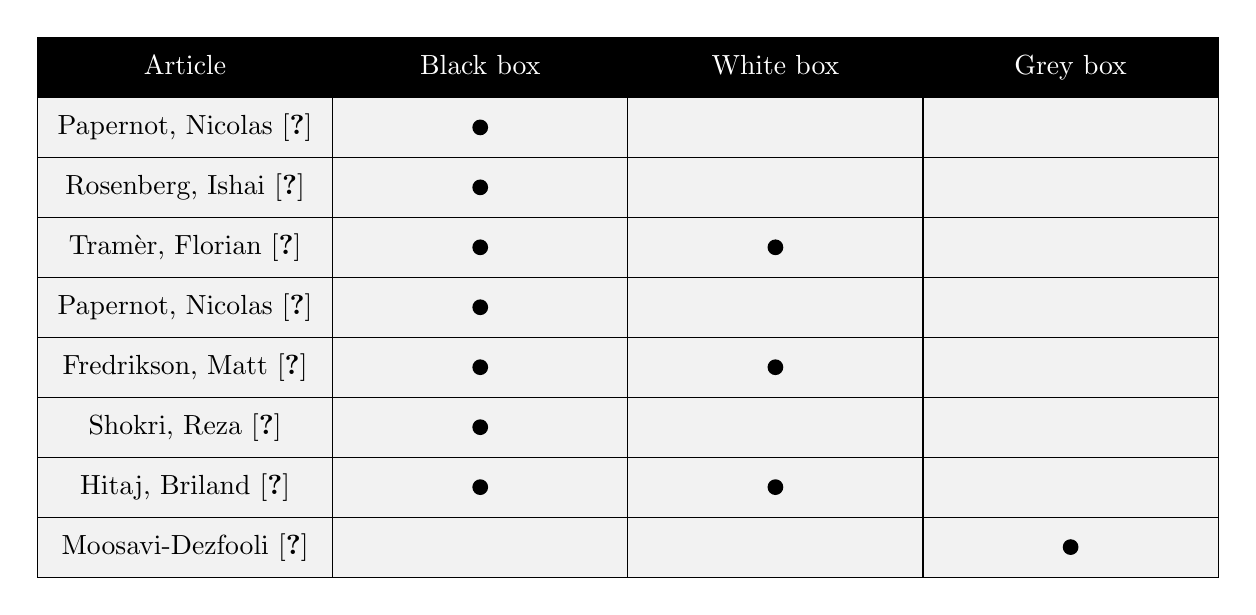
\begin{tikzpicture}
    \matrix[table, rows={2,...,10}{fill=grey!10}, columns={1,...,4}{text width = 8em}, ampersand replacement=\&] (first)
    { 
        Article \& Black box\& White box\& Grey box\\
        Papernot, Nicolas\cite{papernot2016transferability} \& \&  \& \\
        Rosenberg, Ishai \cite{rosenberg2017generic} \& \& \& \\
        Tramèr, Florian \cite{tramer2016stealing} \& \& \& \\
        Papernot, Nicolas \cite{papernot2017practical} \& \& \& \\
        Fredrikson, Matt \cite{fredrikson2015model} \& \& \& \\
        Shokri, Reza \cite{shokri2017membership} \& \& \& \\
        Hitaj, Briland \cite{hitaj2017deep} \& \& \& \\
        Moosavi-Dezfooli \cite{moosavi2016deepfool} \& \& \& \\
};

\fill[black] (first-2-2) circle (\r);
\fill[black] (first-3-2) circle (\r);
\fill[black] (first-4-2) circle (\r);
\fill[black] (first-4-3) circle (\r);
\fill[black] (first-5-2) circle (\r);
\fill[black] (first-6-2) circle (\r);
\fill[black] (first-6-3) circle (\r);
\fill[black] (first-7-2) circle (\r);
\fill[black] (first-8-2) circle (\r);
\fill[black] (first-8-3) circle (\r);
\fill[black] (first-9-4) circle (\r);
\end{tikzpicture}
\caption{Overview of attacks in relevant articles}
\label{tab:table2}
\end{figure}

\begin{table}[h!]
	\centering
	\begin{tabular}{l|c|V}
		Articles & Attacks & Applications\\
		\hline
		Dalvi, Nilesh \cite{dalvi2004adversarial} & Adversarial Classification, & Email Spam detection, fraud \\Biggio, Battista \cite{biggio2008adversarial}, \cite{biggio2014security} & Pattern recognition & detection, intrusion detection, \\ & & biometric identification\\
        \hline
    Papernot, Nicolas & Adversarial samples crafting, & digit recognition, black-box attacks \\ \cite{papernot2017practical}, \cite{papernot2016transferability} & Black box attack & against classifiers hosted by Amazon\\ & on classifiers &and Google \\
    \hline
    Hitaj, Briland \cite{hitaj2017deep} & GAN: Collaborative deep & Access to sensitive information\\ & learning attacks: Black-box & Attack proved effective even against\\ & and white-box attacks & Convolutional Neural Networks which are
     notoriously difficult to invert\\
     \hline
    Moosavi-Dezfooli \cite{moosavi2016deepfool} & Efficiently compute & Image classification \\ & perturbations that fool \\ & deep networks 
    
    \end{tabular}
    \caption{Overview of Attacks and Applications}
	\label{tab:table3}
\end{table}

\subsection*{Adversarial training and attacks}
Adversarial training is a computational method of developing robust DNN models so that a slight perturbation in the input does not mislead a model generating false outputs. A lot of adversarial examples are generated and the model is explicitly trained not to be fooled by each of them. We have discussed this approach in detail in Section \ref{training}. 

Adversarial examples are crafted inputs to the learning model that the attacker meticulously design to cause the model to mistake. Although a lot of promising work in adversarial training has been done, it remains impossible defend a model as it is difficult to construct a theoretical model of the adversarial crafting process. Different attacking methods have been discussed in the following sections. 

\section{Adversarial Training}\label{training}
\cite{wang2016learning} propose a general framework to facilitate the development of adversary resistant DNNs.

	
\subsection{Generating Adversarial Samples}
Adversarial samples are generated by computing the derivative of the cost function with respect to the network’s input variables. The gradient of any input sample represents a direction vector in the model’s high-dimensional input space. Along this direction, a small change in this input sample can cause the DNN to generate a completely different prediction result. This particular direction is important since it represents the most effective way one might compromise the optimization of the cost function. Discovering this particular direction is realized by transmitting the error gradients from output layer all the way back to the input layer via back-propagation. The gradient with respect to the input may then be applied to the input sample(s) to craft an adversarial example(s). We now formally present the generation of adversarial samples by first defining the function g for generating any adversarial sample $\hat{x}$:

\begin{equation}
g : R\textsuperscript{m} \times R\textsuperscript{k} \rightarrow R\textsuperscript{m}
\end{equation}

\begin{equation*}
x \times y \rightarrow \hat{x}
\end{equation*}

where
\begin{equation}\label{4}
\hat{x} = arg \ max \ L(f(\hat{x}), y) \ s.t \ ||\hat{x}-x||_p < \epsilon
\end{equation} and $||.||_p$ is p-norm.
	
Note that g is a one-to-one mapping, meaning that when there exist multiple $\hat{x}$ satisfying \eqref{4}, only one is chosen. It should be noted that the constraint in \eqref{4} ensures that the distortion incurred by manipulation must be maintained at a small scale. Otherwise a significant distortion will leave the manipulation to be easily detected. Existing attacks \cite{carlini2017towards}, \cite{szegedy2013intriguing}, \cite{papernot2016limitations} consist of different approaches for generating adversarial samples which ultimately, can all be described solving following optimization problem, which is a transformation of \eqref{4}:

\begin{equation}\label{5}
	\hat{x}: min c*||x - \hat{x}||_p - L(f(\hat{x}), y)
\end{equation}

where c is some weight or coefficient. Here we refer to this type of attack as an optimal attack, and, for simplicity, denote $||x − \hat{x}||_p$ as the $l_p$ distance. Solving \eqref{5} is done much like solving for the weight coefficients of a standard DNN. Simply put, an attacker can use back-propagation and either gradient descent \cite{szegedy2013intriguing} or L-BFGS \cite{carlini2017towards}. In order to conduct the calculation, one first computes $\partial^n L(f(\hat{x}, y)) / \partial \hat{x}^n$ and then use it for manipulating legitimate samples x. Note that here n = 1 if we use a first-order optimization method like gradient descent, or n = 2 if we utilize a second-order method such as the Newton–Raphson method. Since gradient descent requires an iterative calculation, it can be computationally expensive when the number of adversarial samples to be generated is large. To mitigate this problem, \cite{szegedy2013intriguing} proposed the fast gradient sign method to approximate this iterative calculation where one could use a single step of gradient descent, as follows:

\begin{equation}
	\hat{x} = x + \epsilon . sign(\nabla L(f(x), y))
\end{equation}

where $\epsilon$ is set to control the scale of the distortions applied. Optimal attacks can be generalized to fast gradient sign attacks by selecting the $l_\infty$ distance. In \cite{szegedy2013intriguing}, the authors study an equivalent optimization problem to \eqref{5} by setting p = 2. Another type of attack, as described in \cite{papernot2016limitations}, generates adversarial samples using a greedy approach to solve \eqref{5} and sets p = 0. More specifically, adversarial samples are crafted by iteratively perturbing one coordinate of x at a time. A coordinate is picked by determining by its influence on the final cost.
	
\section{Attacks}\label{attacks}
\ach{the term "adversarial attack" is confusing. Adversary will of course attack. Need to propose a better idea.}
\subsection{Model Inversion(MI) Attack}
\cite{wang2016learning} explains this attack. Once the network has been trained, the gradient can be used to adjust the weights of the network and obtain a reverse-engineered example for all represented classes in the network. For those classes that it did not have prior information, it would still be able to recover prototypical examples. This attack shows that any accurate deep learning machine, no matter how it has been trained, can leak information about the different classes that it can distinguish.
\cite{fredrikson2015model} developed new model inversion attacks through ML APIs that exploit confidence values in a variety of settings and explored countermeasures as simple variant of CART in both black box and white box settings.

\paragraph{Applications} This attack has been successfully experimented in face recognition where \cite{fredrikson2015model} showed given access to the model and person's name, it can recover the facial image, lifestyle prediction, medical genome prediction.

\paragraph{Limitation}: Due to the rich structure of deep learning machines, the model inversion attack may recover only prototypical examples that have little resemblance to the actual data that defined that class. It may or may not be considered as an attack as it may construct wrong/meaningless information.
 
\subsection{Generative Adversarial Attack(GAN)} 
The GAN procedure pits a discriminative deep learning network against a generative deep learning network. The discriminative network is trained to distinguish between images from an original database and those generated by the GAN. The generative network is first initialized with random noise, and at each iteration, it is trained to mimic the images in the training set of the discriminative network. The procedure ends when the discriminative network is unable to distinguish between samples from the original database and the samples generated by the generative network.

\subsection{Black Box and White box attacks}
There are two main research directions in the literature on adversarial attacks based on different assumptions about the adversarial knowledge of the target network. The first and the most common line of work; whitebox attacks assumes that the adversary has detailed knowledge of the network architecture and the parameters resulting from training (or access to the labeled training set). Using this information, an adversary constructs a perturbation for a given image. The most effective methods are gradient-based: a small perturbation is constructed based on the gradient of the network loss function w.r.t. the input image. Often, adding this small perturbation to the original image leads to a misclassification. In the second line of work; black-box attacks, an adversary has restricted knowledge about the network from being able to only observe the network’s output on some probed inputs. This attack strategy is based the idea of greedy local search, an iterative search procedure, where in each round a local neighborhood is used to refine the current image and in process optimizing some objective function that depends on the network output. In each round, the local search procedure generates an implicit approximation to the actual gradient w.r.t the current image by observing changes in output. This approximate gradient provides a partial understanding of the influential pixels in the current image for the output, which is then used to update this image.

\ach{Note: Different examples to be added from \cite{rosenberg2017generic}}

\subsection{Membership Inference Attack}
\ach{To be added from \cite{shokri2017membership}}

\subsection{Gray Box Attacks}
\ach{To be added from \cite{moosavi2016deepfool}}

\section{Adversarial Learning and Attack Strategy (by Manaar)}

\section{Conclusion and Future Challenges}

\bibliographystyle{unsrt}
\bibliography{ref_ml}

\end{document}
